\section{Filter}
\textbf{HAREC a.\ref{HAREC.a.3.2}\label{myHAREC.a.3.2}, a.\ref{HAREC.a.3.2.9}\label{myHAREC.a.3.2.9}}
\index{filter}
\index{filter!frekvensfilter}
\index{frekvensgång}
\index{filter!frekvensgång}
\index{frequency responce}

Frekvensfilter, eller mer allmänt \emph{filter}, används inom radiotekniken för
många olika ändamål, t.ex. för att
\begin{itemize}
  \item eliminera störande signaler
  \item öka avstämningsskärpan (selektiviteten) i mottagare och sändare
  \item framhäva eller dämpa ett sidband i en AM-signal m.m.
\end{itemize}

\emph{Frekvensgången} (eng. \emph{frequency responce}) är ett mått på ett
filters förmåga att släppa igenom olika mycket av olika frekvenser.
Frekvensgången presenteras i allmänhet som en kurva med amplitud av genomsläppt
sinus-signal som funktion av frekvensen.

Beroende på den s.k. frekvensgången, så indelas filtren i flera ''familjer'',
varav de vanligaste presenteras här.

Beroende på det tekniska utförandet finns dels s.k. passiva filter vilka
använder extern energi för sin funktion, och dels aktiva filter vilka i princip
är förstärkare som likaledes använder passiva kretsar.
Här presenteras för enkelhetens skull passiva filter.

Traditionella frekvensfilter är vad som kallas analoga.
Men nu i dataåldern börjar även digitala filter vinna intåg.
Sådana är dock för komplicerade för att behandlas här.

\subsection{Högpassfilter (HP)}
\textbf{HAREC
  a.\ref{HAREC.a.3.2.8b}\label{myHAREC.a.3.2.8b},
  a.\ref{HAREC.a.3.2.9}\label{myHAREC.a.3.2.9a}
}
\index{högpassfilter}
\index{filter!högpass (HP)}
\index{highpass filter}
\index{HP}

\begin{figure}
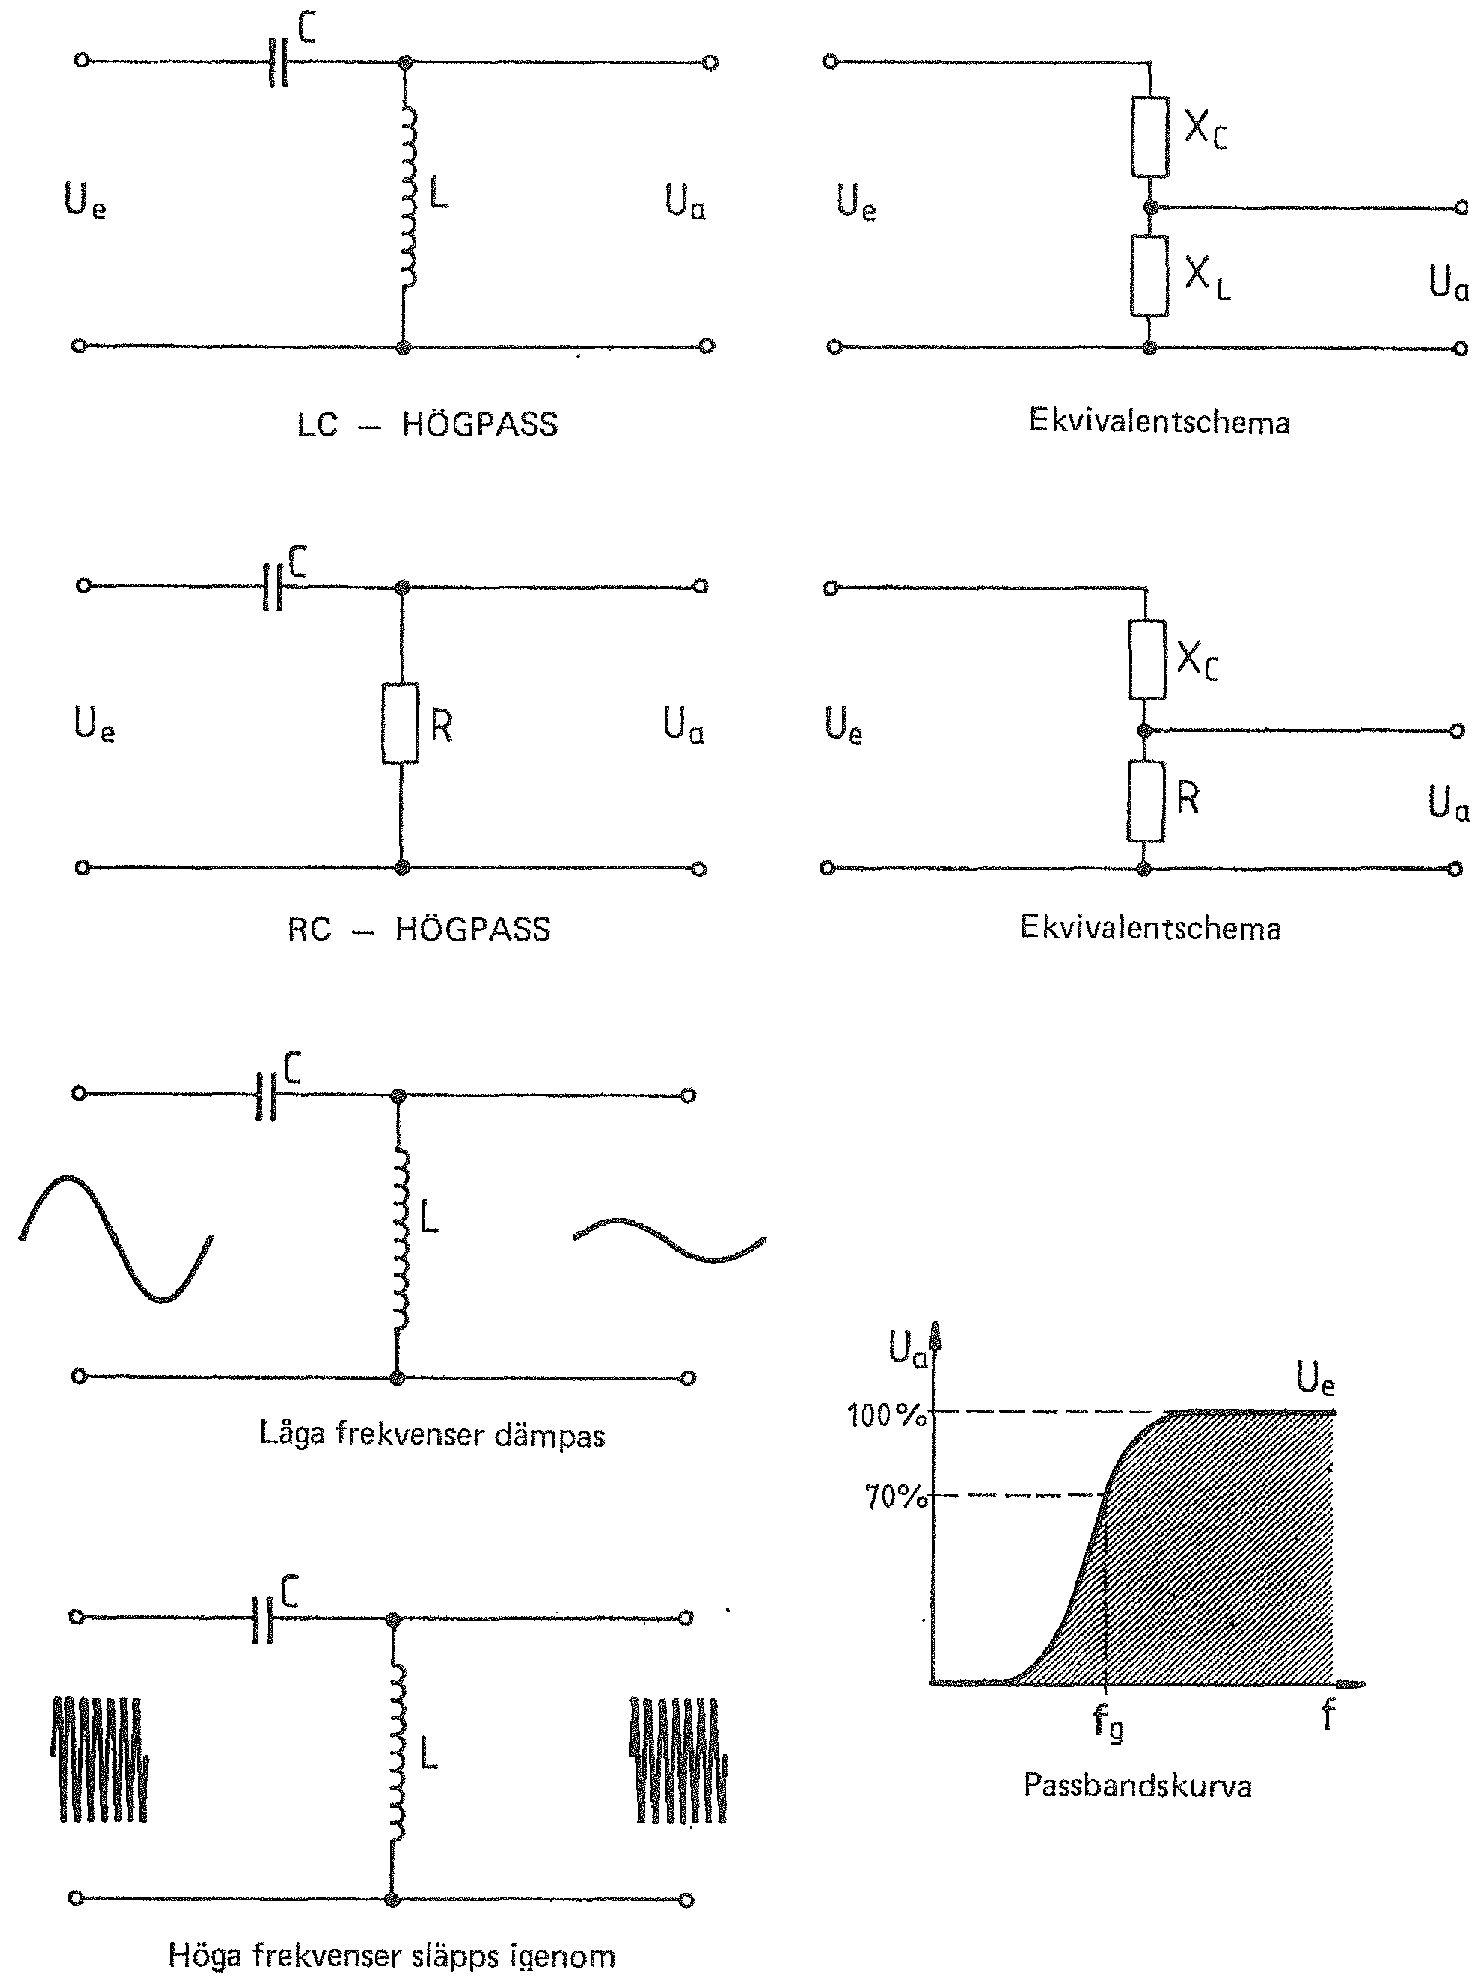
\includegraphics[width=\textwidth]{images/cropped_pdfs/bild_2_3-22.pdf}
\caption{Högpassfilter}
\label{fig:BildII3-22}
\end{figure}

Bild \ref{fig:BildII3-22}

Ett \emph{högpassfilter} (eng. \emph{highpass filter (HP)}) släpper igenom
signaler med höga frekvenser och dämpar dem med låga frekvenser.

\textbf{Exempel:} En frekvensberoende spänningsdelare som LC-högpassfilter.

Vid låga frekvenser är \(X_C\) stor och \(X_L\) liten.
Över XL uppstår då ett litet spänningsfall -- en låg utgångsspänning \(U_a\).
Resultatet blir att låga frekvenser dämpas.

Vid höga frekvenser är \(X_C\) liten och \(X_L\) stor.
Över \(X_L\) uppstår då ett stort spänningsfall -- en hög utgångsspänning
\(U_a\).
Resultatet blir att höga frekvenser släpps igenom.

\(X_L\) kan bytas ut mot en resistor \(R\), men då blir passbandkurvan inte så
brant.

\textbf{Gränsfrekvens}

Gränsfrekvensen \(f_g\) beror av kapacitansen \(C\), induktansen \(L\) samt
resistansen \(R\).

\textbf{LC-högpass:}
\begin{gather*}
  f_g = \frac{1}{2\pi \sqrt{LC}} \\
  f_g\ \text{[Hz]} \quad L\ \text{[H]} \quad C\ \text{[F]}
\end{gather*}

\textbf{RC-Högpass:}
\begin{gather*}
  f_g = \frac{1}{2\pi RC}\\
  f_g\ \text{[Hz]} \quad R\ [\Omega] \quad C\ \text{[F]}
\end{gather*}

\textbf{Räkneexempel:}
\begin{enumerate}
\item \(L = 4\ \text{H} \quad C = 1\ \mu\text{F} \quad f_g =\ ?\)
  \[
  f_g = \frac{1}{2\pi \sqrt{4 \cdot 10^{-6}}} = \frac{500}{2\pi }
  = 79,6\ \text{Hz}
  \]
\item \(R = 1\ k\Omega \quad C = 10\ \text{nF} \quad f_g =\ ?\)
  \[
    f_g = \frac{1}{2\pi  \cdot 1 \cdot 10^3 \cdot 10 \cdot 10^{-9}}
    = \frac{10^5}{2\pi } = 15,9\ \text{kHz}
  \]
\end{enumerate}

\subsection{Lågpassfilter (LP)}
\textbf{HAREC
  a.\ref{HAREC.a.3.2.8a}\label{myHAREC.a.3.2.8a},
  a.\ref{HAREC.a.3.2.9}\label{myHAREC.a.3.2.9b}
}
\index{lågpassfilter}
\index{filter!lågpass (LP)}
\index{lowpass filter}
\index{LP}

\begin{figure}
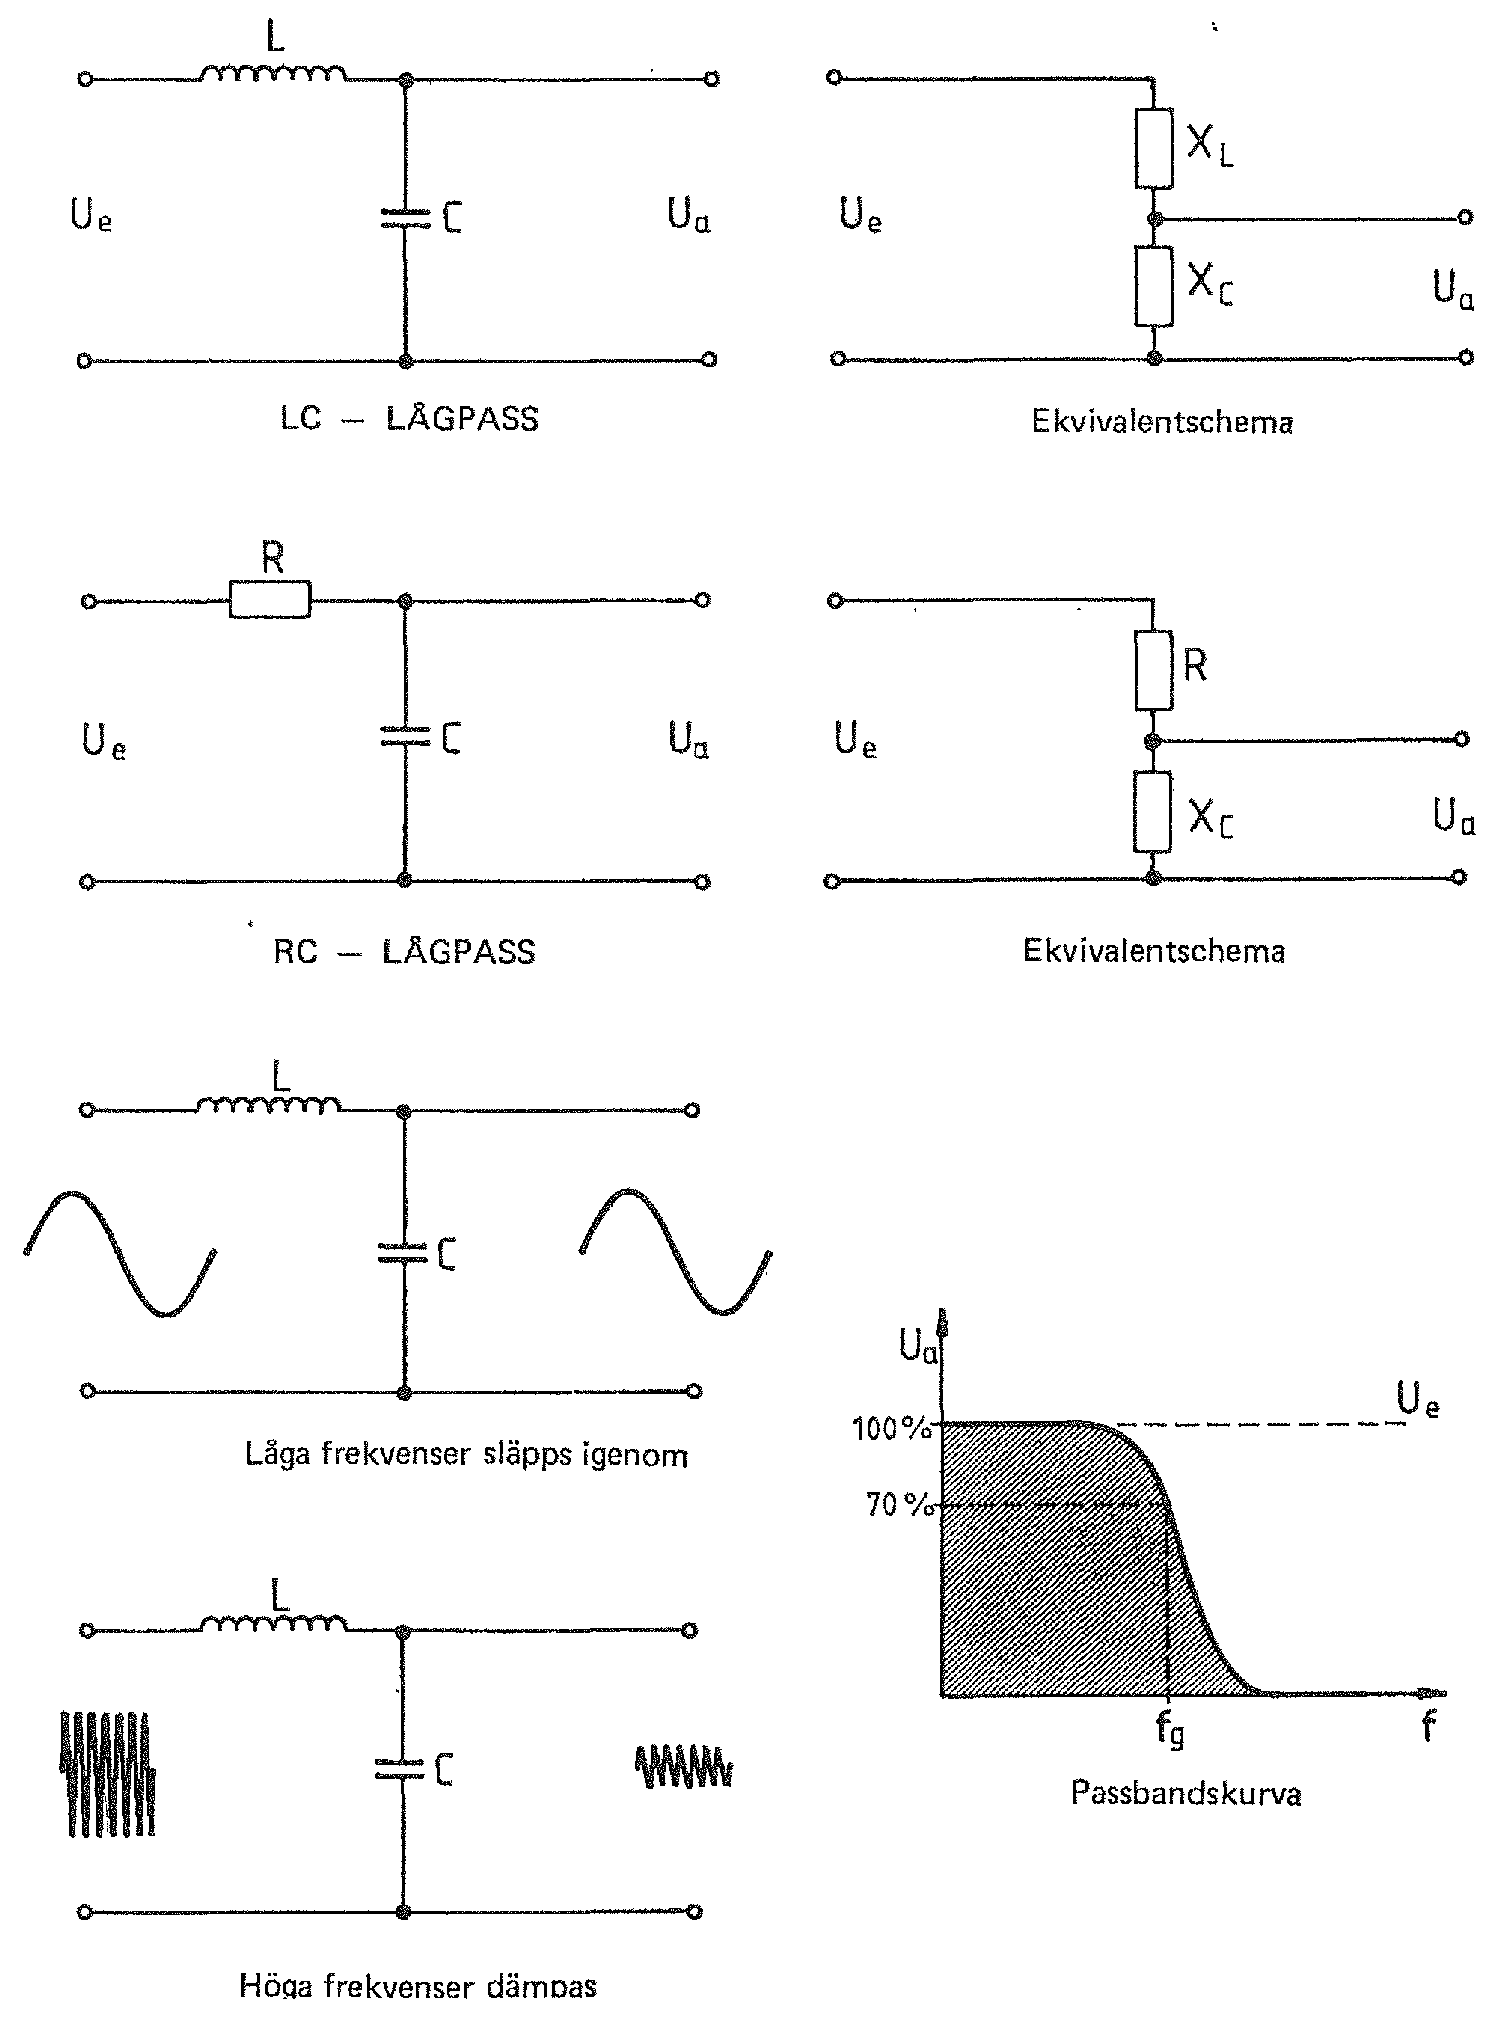
\includegraphics[width=\textwidth]{images/cropped_pdfs/bild_2_3-23.pdf}
\caption{Lågpassfilter}
\label{fig:BildII3-23}
\end{figure}

Om induktor och kondensator respektive resistor och kondensator i ett
högpassfilter byter plats, som i bild \ref{fig:BildII3-23}, så får man i
stället ett LC-lågpassfilter respektive ett RC-lågpassfilter.

Ett \emph{lågpassfilter} (eng. \emph{lowpass filter (LP)}) släpper igenom
signaler med låga frekvenser och dämpar dem med höga frekvenser.

\textbf{Exempel:} En frekvensberoende spänningsdelare som LC-Lågpassfilter.

Vid låga frekvenser är \(X_C\) stor och \(X_L\) liten.
Över \(X_L\) uppstår då ett litet spänningsfall -- en hög utgångsspänning
\(U_a\).
Resultatet blir att låga frekvenser släpps igenom.

Vid höga frekvenser är \(X_C\) liten och \(X_L\) stor.
Över \(X_L\) uppstår då ett stort spänningsfall -- en låg utgångsspänning
\(U_a\).
Resultatet blir att höga frekvenser dämpas.

\textbf{Gränsfrekvens}

Samma formler används vid beräkning av gränsfrekvensen både i lågpass- och
högpassfilter, således

\textbf{LC-Lågpass:}
\begin{gather*}
  f_g = \frac{1}{2\pi \sqrt{LC}} \\
  f_g\ \text{[Hz]} \quad L\ \text{[H]} \quad C\ \text{[F]}
\end{gather*}

\textbf{RC-Lågpass:}
\begin{gather*}
  f_g = \frac{1}{2\pi {RC}} \\
  f_g\ \text{[Hz]} \quad R\ [\Omega] \quad C\ \text{[F]}
\end{gather*}

\subsection{Bandpassfilter (BP)}
\textbf{HAREC
  a.\ref{HAREC.a.3.2.7}\label{myHAREC.a.3.2.7},
  a.\ref{HAREC.a.3.2.8c}\label{myHAREC.a.3.2.8c},
  a.\ref{HAREC.a.3.2.9}\label{myHAREC.a.3.2.9c}
}
\index{bandpassfilter}
\index{filter!bandpass (BP)}
\index{bandpass filter}
\index{BP}

\begin{figure}
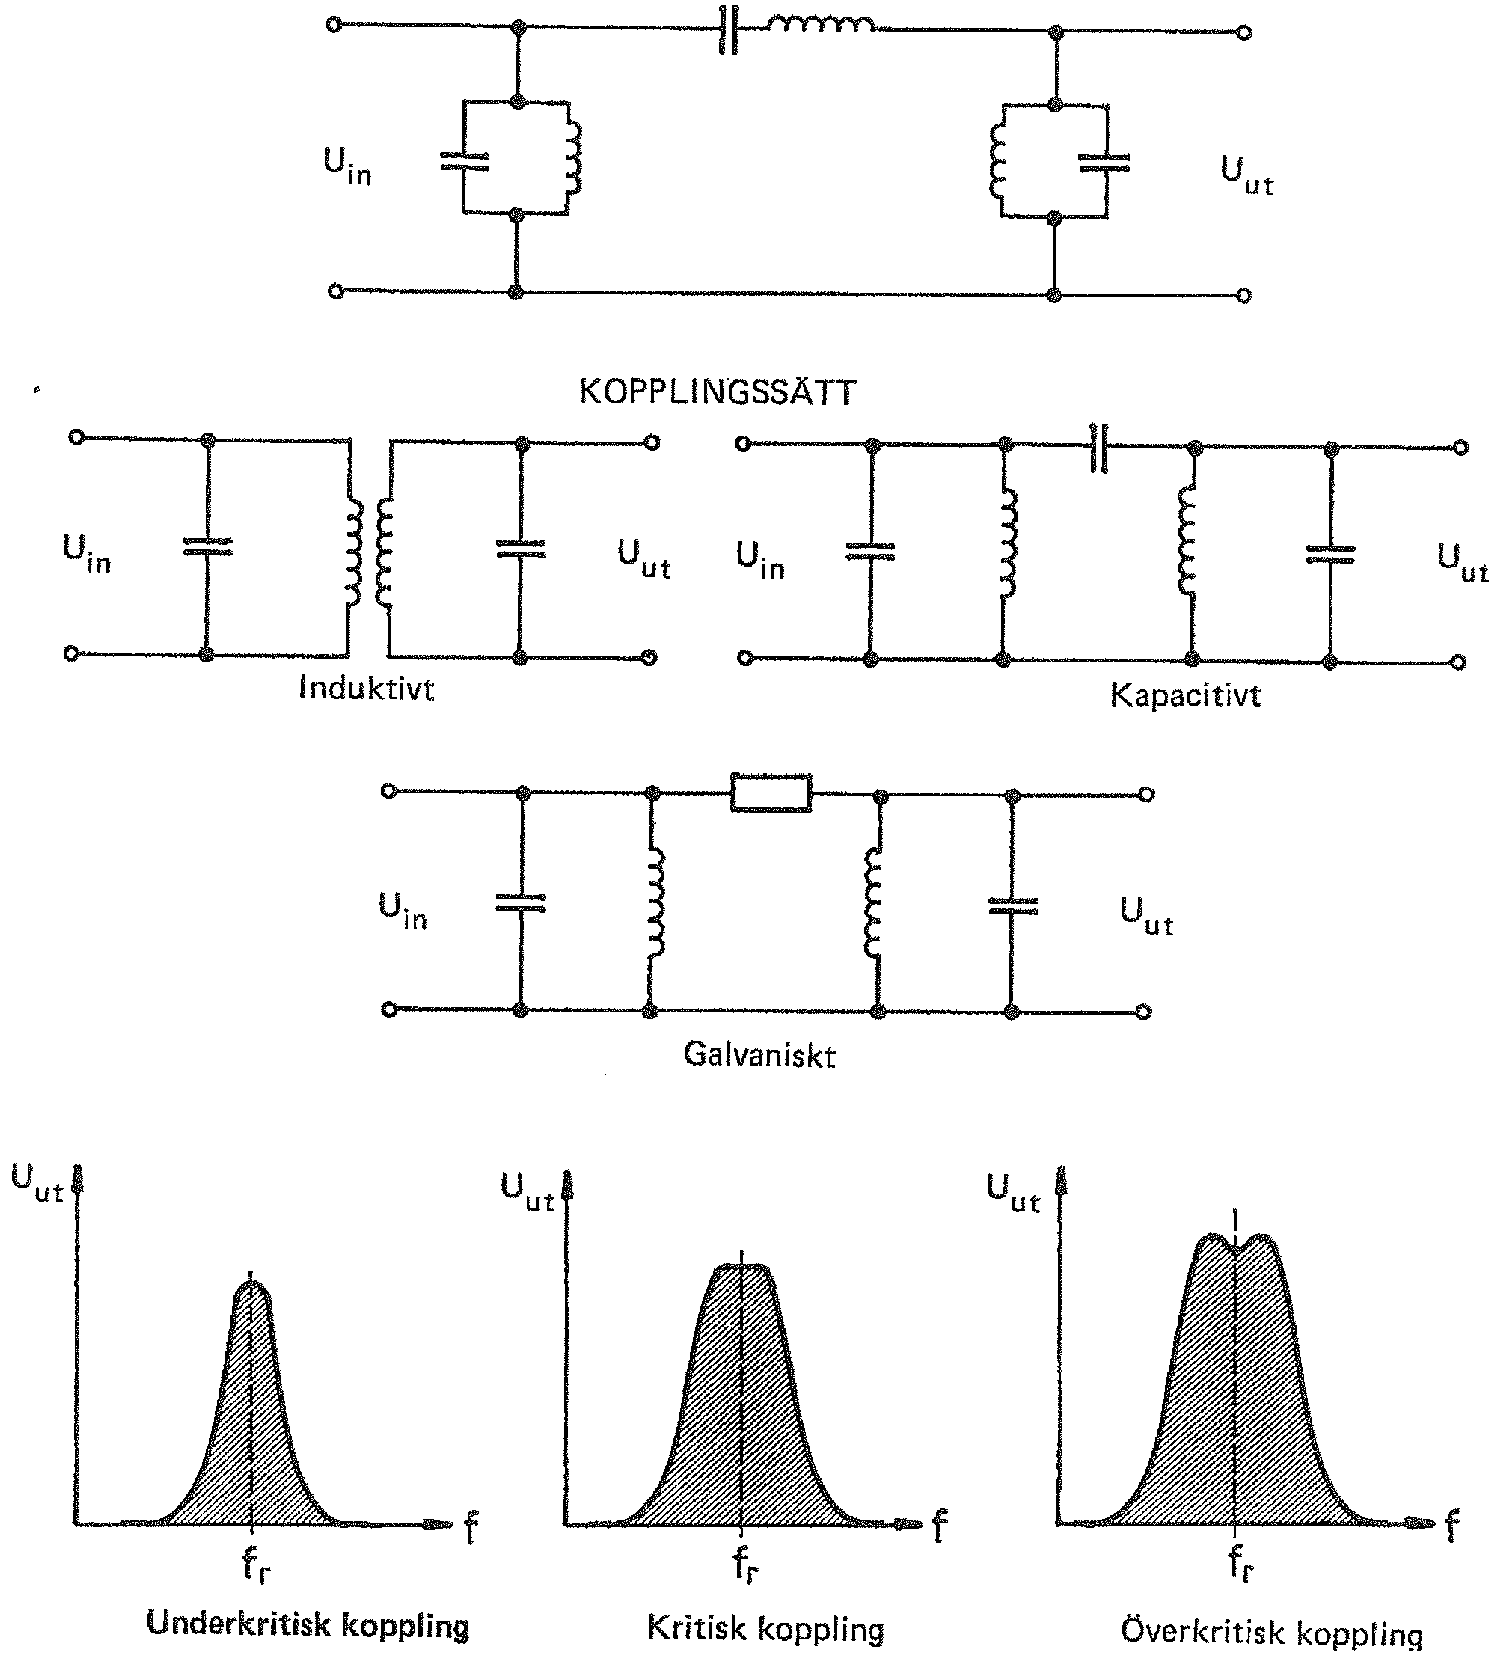
\includegraphics[width=\textwidth]{images/cropped_pdfs/bild_2_3-24.pdf}
\caption{Bandpassfilter}
\label{fig:BildII3-24}
\end{figure}

Ett \emph{bandpassfilter} (eng. \emph{bandpass filter}) släpper igenom signaler
bara inom ett frekvensområde medan signaler inom andra frekvensområden dämpas.

Bandpassfiltret består i enklaste fall av två svängningskretsar av LC-typ, vilka
är avstämda till angränsande frekvenser. Kretsarna är kopplade induktivt,
kapacitivt eller galvaniskt så som illustreras i bild \ref{fig:BildII3-24}.

Beroende på kopplingsgrad eller dämpning skiljer man mellan underkritisk
koppling (lös koppling), kritisk koppling och överkritisk koppling
(fast koppling).

På bilden visas hur passbandet påverkas bl.a. av kopplingsgraden.
Lös koppling liten bandbredd.
Kritisk koppling -- större bandbredd.
Fast koppling -- stor bandbredd.

\subsection{Passfilter}
\textbf{HAREC
  a.\ref{HAREC.a.3.2.9}\label{myHAREC.a.3.2.9d}
}
\index{passfilter}
\index{filter!bandpass (BP)}
\index{pass filter}
\index{BP}

\begin{figure}
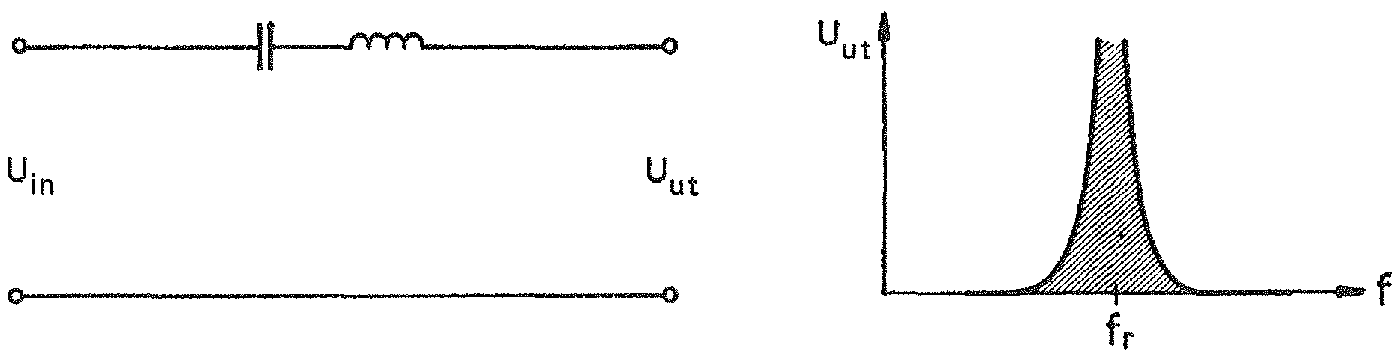
\includegraphics[width=\textwidth]{images/cropped_pdfs/bild_2_3-25.pdf}
\caption{Passfilter}
\label{fig:BildII3-25}
\end{figure}


Passkretsen eller passfilter stäms av till en viss frekvens och erbjuder där
en mycket låg impedans så som illustreras i bild \ref{fig:BildII3-25}.
Passkretsen kopplas i serie med signalvägen och låter signaler med
frekvenser inom filtrets passband att passera.

\subsection{Bandspärrfilter}
\textbf{HAREC
  a.\ref{HAREC.a.3.2.8d}\label{myHAREC.a.3.2.8d},
  a.\ref{HAREC.a.3.2.9}\label{myHAREC.a.3.2.9e}
}
\index{bandspärrfilter}
\index{filter!bandspärr (BR)}
\index{band reject filter (BR)}
\index{BR}

\begin{figure}
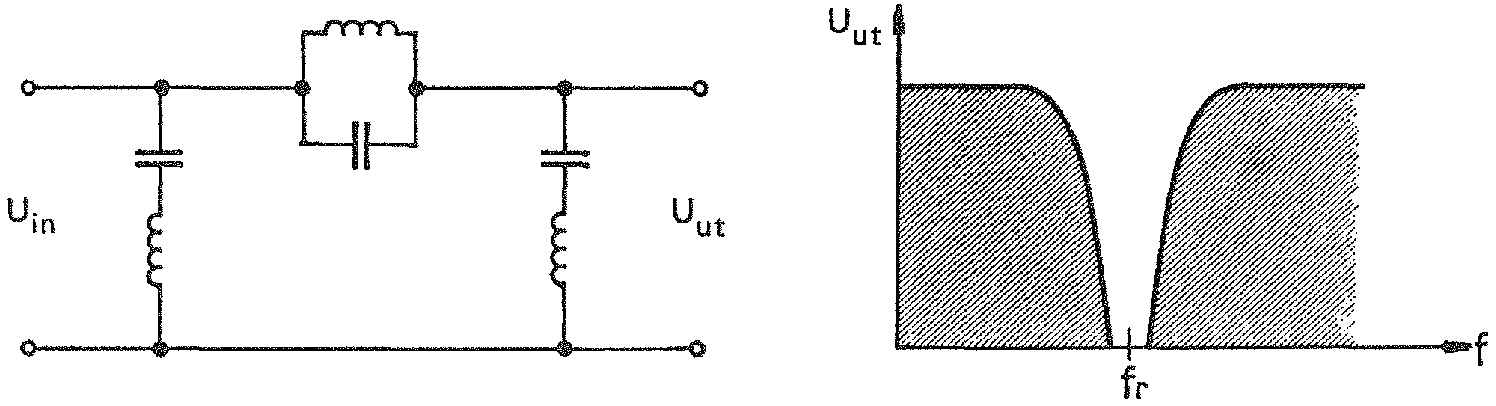
\includegraphics[width=\textwidth]{images/cropped_pdfs/bild_2_3-26.pdf}
\caption{Bandspärrfilter}
\label{fig:BildII3-26}
\end{figure}

Om serie- och parallellkretsarna i ett bandpassfilter byter plats, så får man
i stället ett bandspärrfilter så som illustreras i bild \ref{fig:BildII3-26}.
Ett sådant spärrar signaler inom ett visst frekvensområde, men släpper igenom
signaler utom detta område.

\subsection{Spärrfilter}
\index{bandspärrfilter}
\index{filter!bandspärr (BR)}
\index{band reject filter (BR)}
\index{BR}
\index{spärrkrets}
\index{sugkrets}

\begin{figure}
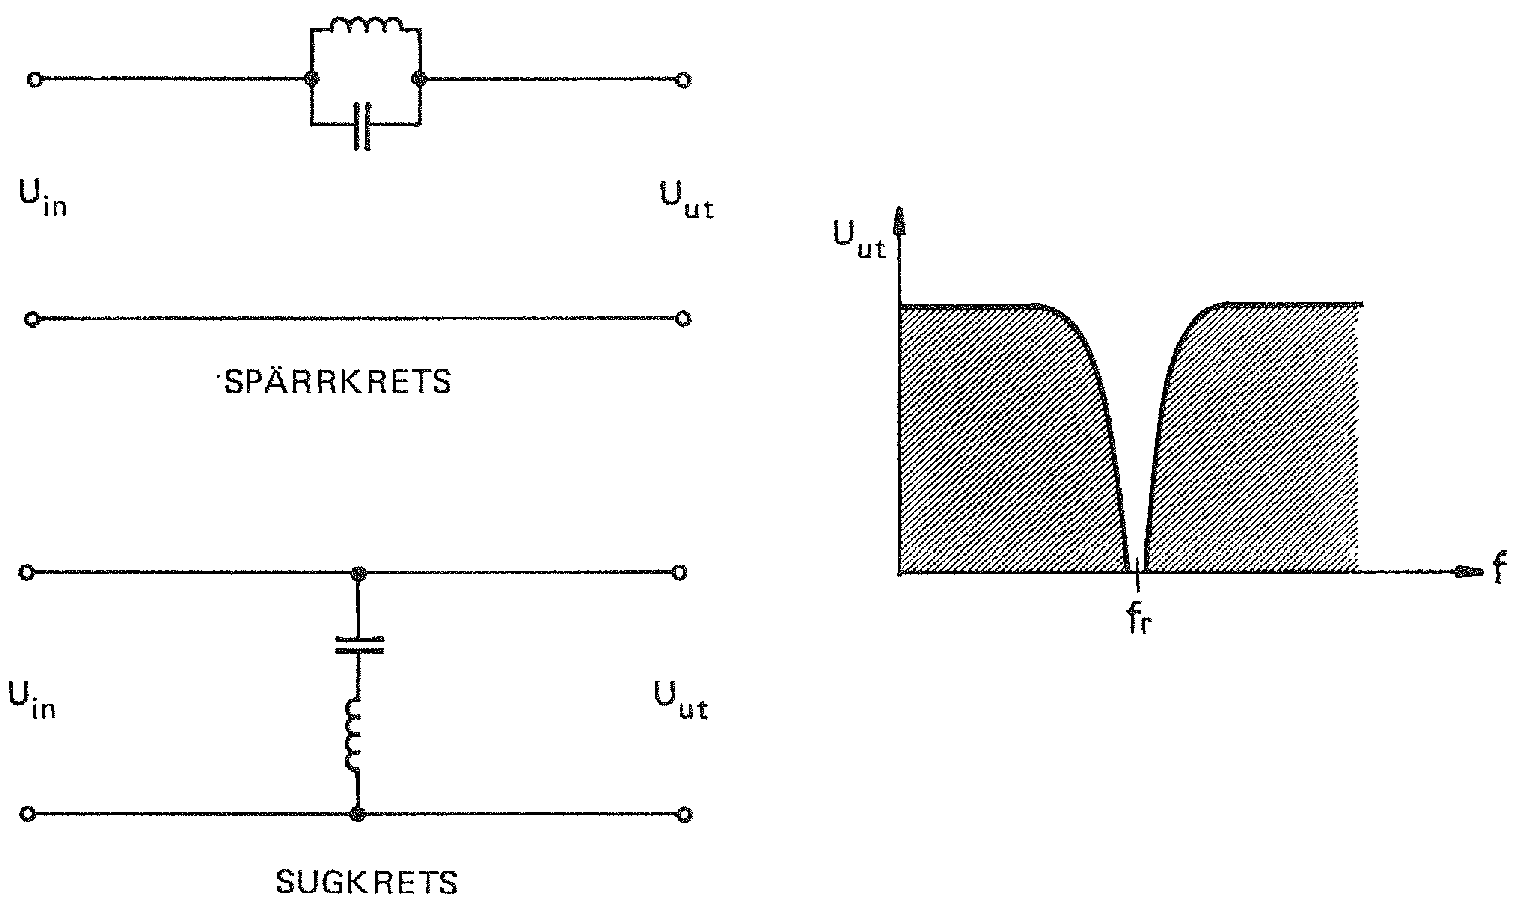
\includegraphics[width=\textwidth]{images/cropped_pdfs/bild_2_3-27.pdf}
\caption{Spärrfilter (2 sorter)}
\label{fig:BildII3-27}
\end{figure}

\subsubsection{Spärrkrets}
Spärrkretsen stäms av till en viss frekvens och erbjuder där en mycket hög
impedans.
Spärrkretsen kopplas i serie med signalvägen och spärrar en signal med samma
frekvens som resonansfrekvensen, så som illustreras i bild \ref{fig:BildII3-27}.

\subsubsection{Sugkrets}
Sugkretsen stäms av till en viss frekvens och erbjuder där en mycket låg
impedans.
Sugkretsen kopplas parallellt med signalvägen och kortsluter (suger bort) en
signal med samma frekvens som resonansfrekvensen, så som illustreras i bild
\ref{fig:BildII3-27}.

\begin{wrapfigure}[14]{R}{0.5\textwidth}
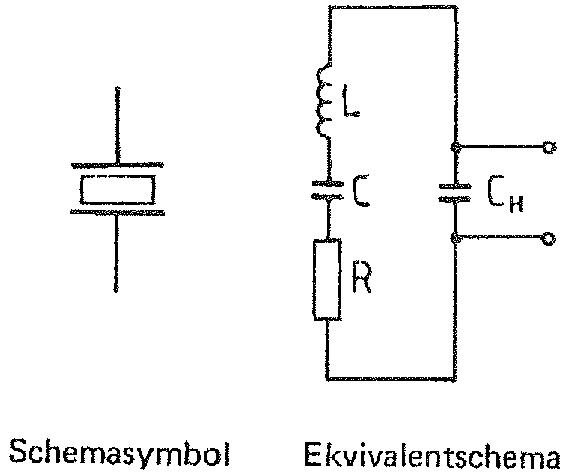
\includegraphics[width=0.5\textwidth]{images/cropped_pdfs/bild_2_3-28.pdf}
\caption{Kvartskristall}
\label{fig:BildII3-28}
\end{wrapfigure}

\subsection{Kvartskristall}

\textbf{HAREC a.\ref{HAREC.a.3.2.11}\label{myHAREC.a.3.2.11}}
\index{kvartskristall}
\index{quartz crystal}
\index{crystal}
\index{Q-värde}
\index{resonator}

En \emph{kvartskristall} (eng. \emph{quartz crystal} eller \emph{crystal}),
egentligen en slipad skiva av kvarts, kan fungera som en
elektromekanisk svängningskropp (resonator), vars egenskaper liknar dem i en
LC-krets.
Detta illustreras i bild \ref{fig:BildII3-28}.

Den låga inre resistansen gör att Q-värdet i en kvartskristall är bättre än
10000.
Som jämförelse är Q-värdet i en LC-krets oftast sämre än 1000.

Många moderna kvartskristaller kan uppvisa olastat Q-värde på 100000.

\vspace{12pt} % Undgår brytning av nästa titelrad

\subsection{Bandfilter med kvartskristaller}
\index{kristallfilter}
\index{crystal filter}
\index{keramiska resonatorer}
\index{ceramic resonators}

\begin{wrapfigure}[17]{R}{0.5\textwidth}
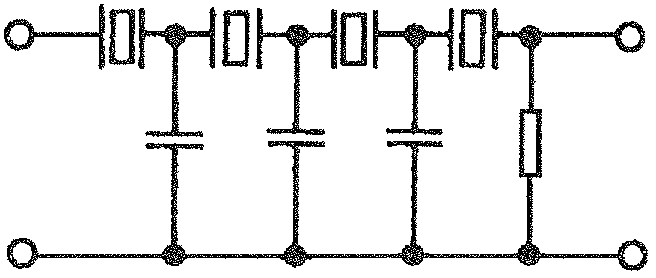
\includegraphics[width=0.5\textwidth]{images/cropped_pdfs/bild_2_3-29.pdf}
\caption{Bandfilter med kvartskristaller}
\label{fig:BildII3-29}
\end{wrapfigure}

Bild \ref{fig:BildII3-29} visar hur kvartskristaller kan kombineras till
filter, ofta refererade till som \emph{kristallfilter} (eng.
\emph{crystal filter}), med önskad bandbredd.
Även utföranden med \emph{keramiska resonatorer} (eng.
\emph{ceramic resonators}) finns.
Resonatorerna är avstämda till var sin bestämda frekvens och hela komplexet
bidrar på så sätt till att bilda passband eller andra egenskaper på samma sätt
som med sammankopplade LC-kretsar.

\subsection{Mekaniska filter}
\index{mekaniskt filter}
\index{mechanical filter}
\index{mekanisk resonator}
\index{resonator!mekanisk}

Med en elektromekanisk givare kan man få en kropp (resonator) att svänga på sin
resonansfrekvens.
Med ännu en elektromagnetisk givare kan man känna av svängningarna och
återvandla dem till elektriska signaler.
Bild \ref{fig:BildII3-30} illustrerar ett sådant arrangemang.
Hela anordningen fungerar som en \emph{elektromekanisk resonator} (eng.
\emph{mechanical resonator}), vars egenskaper liknar dem i en LC-krets.

\begin{figure}
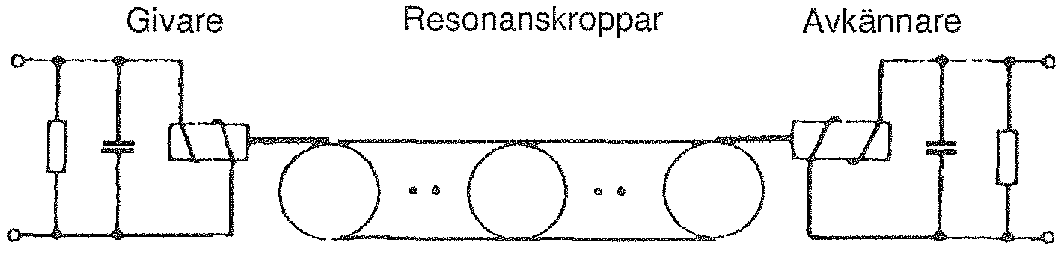
\includegraphics[width=\textwidth]{images/cropped_pdfs/bild_2_3-30.pdf}
\caption{Mekaniskt filter}
\label{fig:BildII3-30}
\end{figure}

Resonatorerna kan kombineras till filterkomplex med önskad bandbredd där
resenatorerna är avstämda till var sin bestämda frekvens.
Hela komplexet bidrar på så sätt till att bilda ett passband på samma sätt som
med sammankopplade LC-kretsar.
Beroende på tillämpningen finns olika frekvenslägen i intervallet 60--600~kHz.

\emph{Mekaniska filter} (eng. \emph{mechanical filter}) användes mest förr som
mellanfrekvensfilter i högvärdiga radioutrustningar, men har numera till stor
del ersatts av bandfilter med kvartskristaller där arbetsområdet kan ligga
avsevärt högre i frekvens.

\subsection{Kavitetsfilter}
\index{kavitetsfilter}
\index{cavity filter}
\index{filter!kavitet}

%%\begin{figure*}[ht]
%%\begin{center}
\begin{wrapfigure}[15]{R}{0\textwidth}
  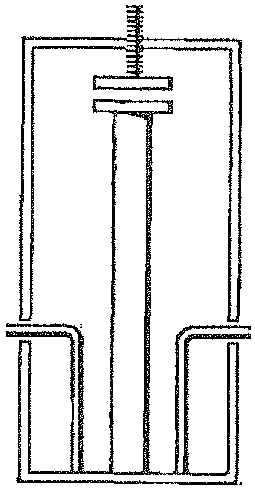
\includegraphics[width=0.2\textwidth]{images/cropped_pdfs/bild_2_3-31.pdf}
  \caption{Kavitetsfilter}
  \label{fig:BildII3-31}
\end{wrapfigure}
%%\end{center}
%%\end{figure*}

Svängningskretsars dimensioner minskar med ökande frekvens.
Vid mycket hög frekvens kan induktorns varvtal i en LC-krets ha minskat till
ett enda varv samtidigt som kapacitansen inom detta enda varv kan räcka för
önskad resonansfrekvens.

En sådan svängningskrets kan bl.a. ha formen av en ledare mitt inne i en
elektriskt ledande kavitet, så som illustreras i bild \ref{fig:BildII3-31}.
Ledarens längd tillsammans med kavitetens insida bildar induktorn.
Mellan ledaren och kavitetens insida råder en kapacitans, som kan
kompletteras/justeras med en extra kondensator.

Inkommande och utgående signaler ansluts till filtrets mittledare över
induktionsslingor, kondensatorer eller direkt galvaniskt.
\emph{Kavitetsfilter} (eng. \emph{cavity filter}) kan kopplas ihop för att
bilda bandfilter, frekvensdelare m.m.

Kavitetsfilter används ofta på sändare eftersom de med sina låga förluster kan
hantera stora effekter samt åstakomma djuppa utsläckningar.
Dessa egenskaper gör dem oerhört lämpliga som duplex filter till repeatrar.

\subsection{Helixfilter}
\index{helixfilter}
%\index{helix filter}
\index{filter!helix}

När ett kompakt kavitetsfilter behövs, så kan man öka reaktansen i mittledaren
både induktivt och kapacitivt genom att utforma den som en spiral (helix).
Detta är dock på bekostnad av Q-värdet.
Flera kavitetsfilter kan kopplas ihop för att bilda bandfilter, spärrfilter m.m.

\subsection{Pi-filter}
\textbf{HAREC a.\ref{HAREC.a.3.2.10a}\label{myHAREC.a.3.2.10a}}
\index{Pi-filter}
\index{filter!Pi-filter}

\begin{wrapfigure}[16]{R}{0.5\textwidth}
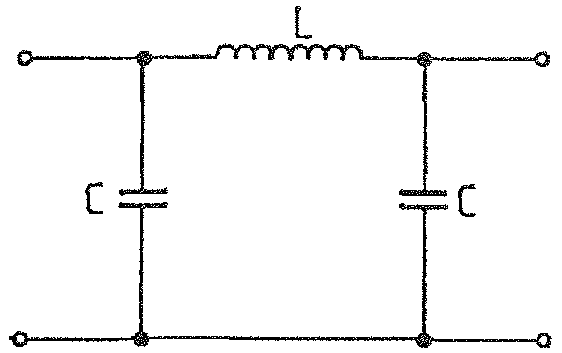
\includegraphics[width=0.5\textwidth]{images/cropped_pdfs/bild_2_3-32.pdf}
\caption{Pi-filter}
\label{fig:BildII3-32}
\end{wrapfigure}

För att överföra HF-signaler med bästa verkningsgrad, så är det viktigt med god
impedansanpassning mellan de olika funktionerna.
Om anslutningsimpedansen är lika i båda funktionerna, så behövs inga extra
åtgärder.
Är impedanserna däremot olika, så behövs korrigeringsnät (filter).

Ofta är nätet Pi-format, så som bild \ref{fig:BildII3-32} visar, och består av
induktanser och kapacitanser.
Ett Pi-format nät kan sägas bestå av två L-formade nät ställda mot varandra, där
den seriella delen är gemensam (på bilden en induktor).

\subsection{T-filter}
\textbf{HAREC a.\ref{HAREC.a.3.2.10b}\label{myHAREC.a.3.2.10b}}
\index{T-filter}
\index{filter!T-filter}

\begin{wrapfigure}[16]{R}{0.5\textwidth}
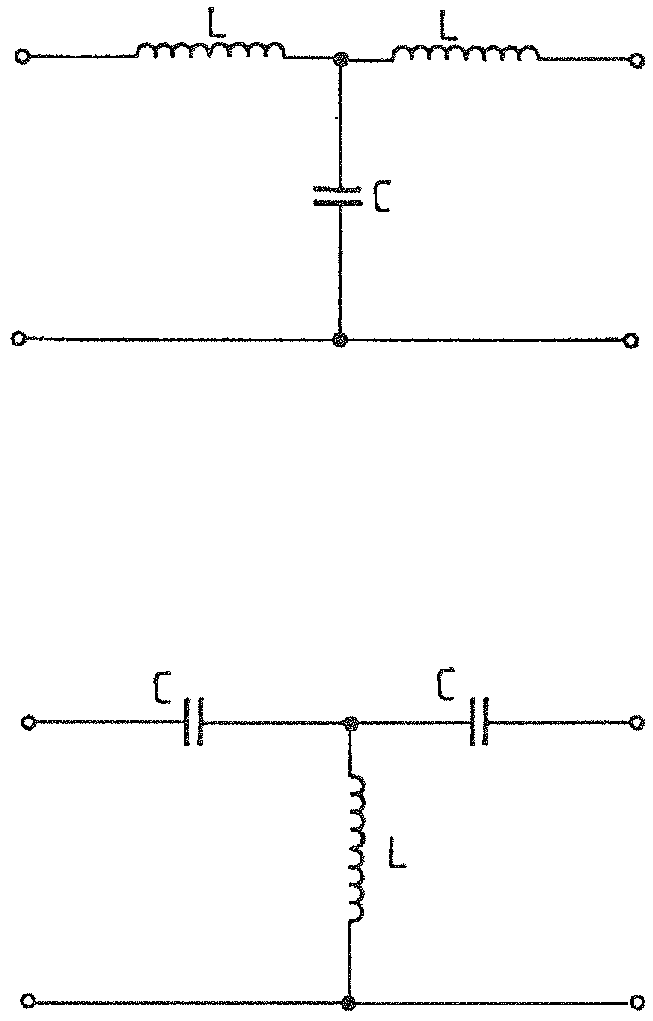
\includegraphics[width=0.5\textwidth]{images/cropped_pdfs/bild_2_3-33.pdf}
\caption{T-filter}
\label{fig:BildII3-33}
\end{wrapfigure}

Ett nät kan också vara T-format, som bild \ref{fig:BildII3-33} visar, och bestå
av induktanser och kapacitanser.
Ett sådant nät kan sägas bestå av två L-formade nät ställda ''rygg mot rygg''.
Då är den parallella delen gemensam.
På bilden visas två alternativ.

När den parallella delen är kapacitiv, blir huvudkaraktären ett lågpassfilter,
men att impedansanpassning också är möjlig med en induktiv impedansdelning.

När den parallell delen är induktiv blir huvudkaraktären ett högpassfilter, men
att impedansanpassning också är möjlig med en kapacitiv impedansdelning.

Ett Pi- eller T-filter kan fungera som
\begin{itemize}
  \item svängningskrets
  \item impedanstransformator (anpassning)
  \item balansera ut en reaktans o.s.v.
\end{itemize}

\subsection{Icke-ideala komponenter}
\textbf{HAREC a.\ref{HAREC.a.3.2.12}\label{myHAREC.a.3.2.12}}

För alla analoga kompoenter så är de verkliga egenskaperna behäftade med
oönskade egenskaper, även kända som parasitiska egenskaper.

Ett motstånd uppvisar inte enbart en strikt resitiv egenskap, utan för högre
frekvenser kommer även en parasitisk seriekopplad induktans göra sig påmind.

En kondensator har inte perfekt isolation, utan det läcker alltid mellan
plattorna med en parasitisk parallelkopplad resistans, som kommer att ladda ur
kondensatorn.

En induktor är inte perfekt förlustfri, utan den har en parasitisk
serieresistans.

För kondensatorer och induktorer kommer resistansen att påverka dess Q-värde,
och ett högt Q-värde anger att man har låg förlust i förhållande till dess
reaktans.
Dessa förluster kommer även göra sig påminda när man bygger kretsar med dessa
komponenter, t.ex. kommer en LC krets i praktiken alltid vara en LCR krets, där
förlusterna i spole och kondensator ger en ekvivalent förlust i kretsen och
sätter en begränsning i hur högt Q-värde den kan uppnå, givet en ideal omvärd.
Vare resonator lastas dock, vilket ytterligare ökar på förlusten och därmed
ytterligare sänker Q-värdet.

\subsection{Digitala filter}
\textbf{HAREC a.\ref{HAREC.a.3.2.13}\label{myHAREC.a.3.2.13}}
\index{digitala filter}

Med den utveckling som skett, kan allt mer processing ske digitalt, det gör
det möjligt att göra \emph{digitala filter}, om bara signalen konveterats till
digital form och sedan konverteras tillbaka till analog form.
Digitala filter har en många fördelar, då man kan göra komplicerade och
skarpa filter som behåller sina egenskaper då den digitala implementationsformen
är stabil över tiden, där klassiska analoga kan behöva trimmas både
individuellt vid tillverkning och över tiden för att upprätthålla sina
egenskaper.

För mer om digitala filter se \ref{DSP} samt \ref{digitala filter}.
